\documentclass[12pt]{article}

\include{preamble}

\newtoggle{professormode}
%\toggletrue{professormode} %STUDENTS: DELETE or COMMENT this line



\title{MATH 342W / 642 / RM 742 Spring \the\year~ HW \#5}

\author{Ye Htut Maung} %STUDENTS: write your name here

\iftoggle{professormode}{
\date{Due 6PM May 16 \\ \vspace{0.5cm} \small (this document last updated \currenttime~on \today)}
}

\renewcommand{\abstractname}{Instructions and Philosophy}

\begin{document}
\maketitle

\iftoggle{professormode}{
\begin{abstract}
The path to success in this class is to do many problems. Unlike other courses, exclusively doing reading(s) will not help. Coming to lecture is akin to watching workout videos; thinking about and solving problems on your own is the actual ``working out.''  Feel free to \qu{work out} with others; \textbf{I want you to work on this in groups.}

Reading is still \textit{required}. You should be googling and reading about all the concepts introduced in class online. This is your responsibility to supplement in-class with your own readings.

The problems below are color coded: \ingreen{green} problems are considered \textit{easy} and marked \qu{[easy]}; \inorange{yellow} problems are considered \textit{intermediate} and marked \qu{[harder]}, \inred{red} problems are considered \textit{difficult} and marked \qu{[difficult]} and \inpurple{purple} problems are extra credit. The \textit{easy} problems are intended to be ``giveaways'' if you went to class. Do as much as you can of the others; I expect you to at least attempt the \textit{difficult} problems. 

This homework is worth 100 points but the point distribution will not be determined until after the due date. See syllabus for the policy on late homework.

Up to 7 points are given as a bonus if the homework is typed using \LaTeX. Links to instaling \LaTeX~and program for compiling \LaTeX~is found on the syllabus. You are encouraged to use \url{overleaf.com}. If you are handing in homework this way, read the comments in the code; there are two lines to comment out and you should replace my name with yours and write your section. The easiest way to use overleaf is to copy the raw text from hwxx.tex and preamble.tex into two new overleaf tex files with the same name. If you are asked to make drawings, you can take a picture of your handwritten drawing and insert them as figures or leave space using the \qu{$\backslash$vspace} command and draw them in after printing or attach them stapled.

The document is available with spaces for you to write your answers. If not using \LaTeX, print this document and write in your answers. I do not accept homeworks which are \textit{not} on this printout. Keep this first page printed for your records.

\end{abstract}

\thispagestyle{empty}
\vspace{1cm}
NAME: \line(1,0){380}
\clearpage
}




\problem{These are some questions related to probability estimation modeling and asymmetric cost modeling. It might be helpful to look back to the review the logistic regression  before doing this problem.}

\begin{enumerate}

\easysubproblem{Graph a canonical ROC and label the axes. In your drawing estimate AUC. Explain very clearly what is measured by the $x$ axis and the $y$ axis.}\spc{7}

\begin{figure}[H]
    \centering
    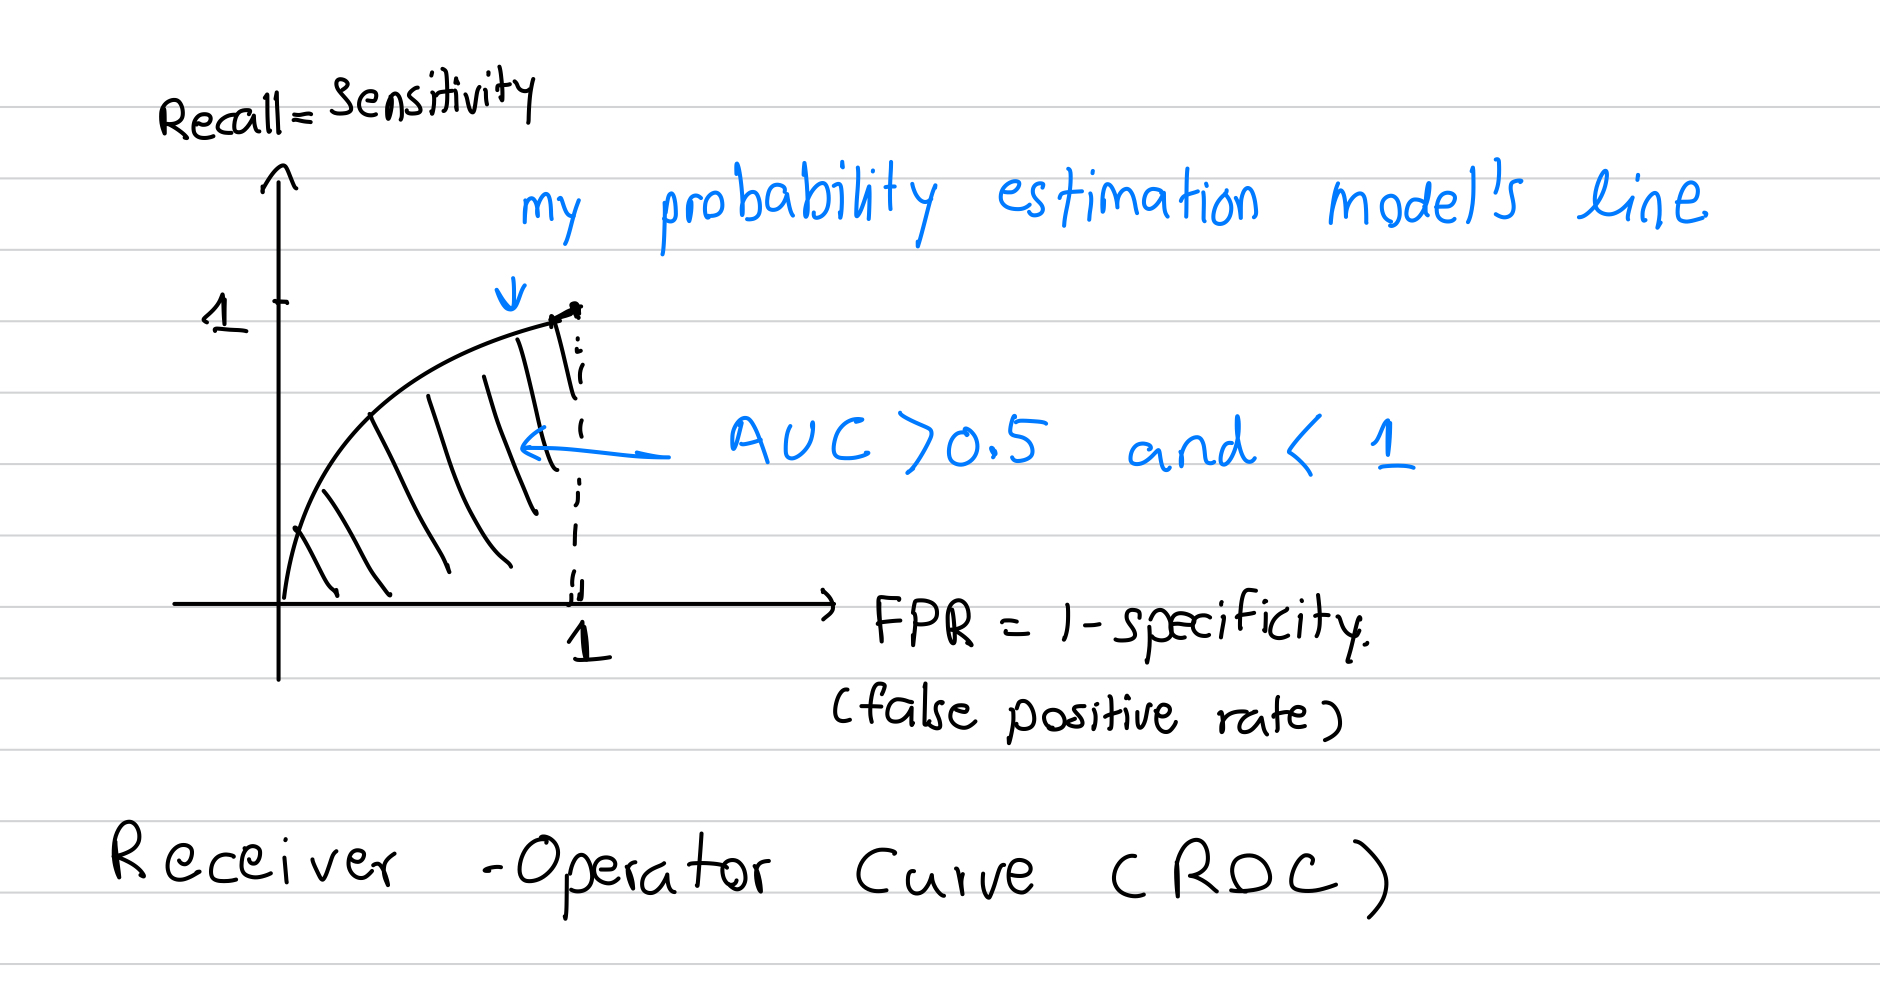
\includegraphics[width=0.75\linewidth]{imgs/img1.jpeg}
    \caption{ROC}
    \label{fig:enter-label}
\end{figure}

X-axis measure how often the model wrongly predicts positive when it's actually negative
Y-axis measure how often the model correctly prediccts positive when it actually is.
Recall is TP/P and FPR is FP/N.
The ROC curve is created by varying the decision threshold $p_{th}$ used to classify a predicted probability as positive. As $p_{th}$ increase, the model becomes more sensitive, increasing both TPR and FPR.

\easysubproblem{Pick one point on your ROC curve from the previous question. Explain a situation why you would employ this model.}\spc{3}

If I select a point with FPR = 0.4 and Recall = 0.6, that corresponds to a particular threshold$ p_{th}$ likely lower than 0.5  that prioritizes catching positives.
This point means the model correctly identifies 60\% of true positives but falsely flags 40\% of true negatives as positives.
I would use such a threshold in situations where false negatives are more costly than false positives, such as in medical diagnostics or fraud detection, where missing a true case is worse than raising a false alarm.

\intermediatesubproblem{Graph a canonical DET curve and label the axes. Explain very clearly what is measured by the $x$ axis and the $y$ axis. Make sure the DET curve's intersections with the axes is correct.}\spc{7}

\begin{figure}[H]
    \centering
    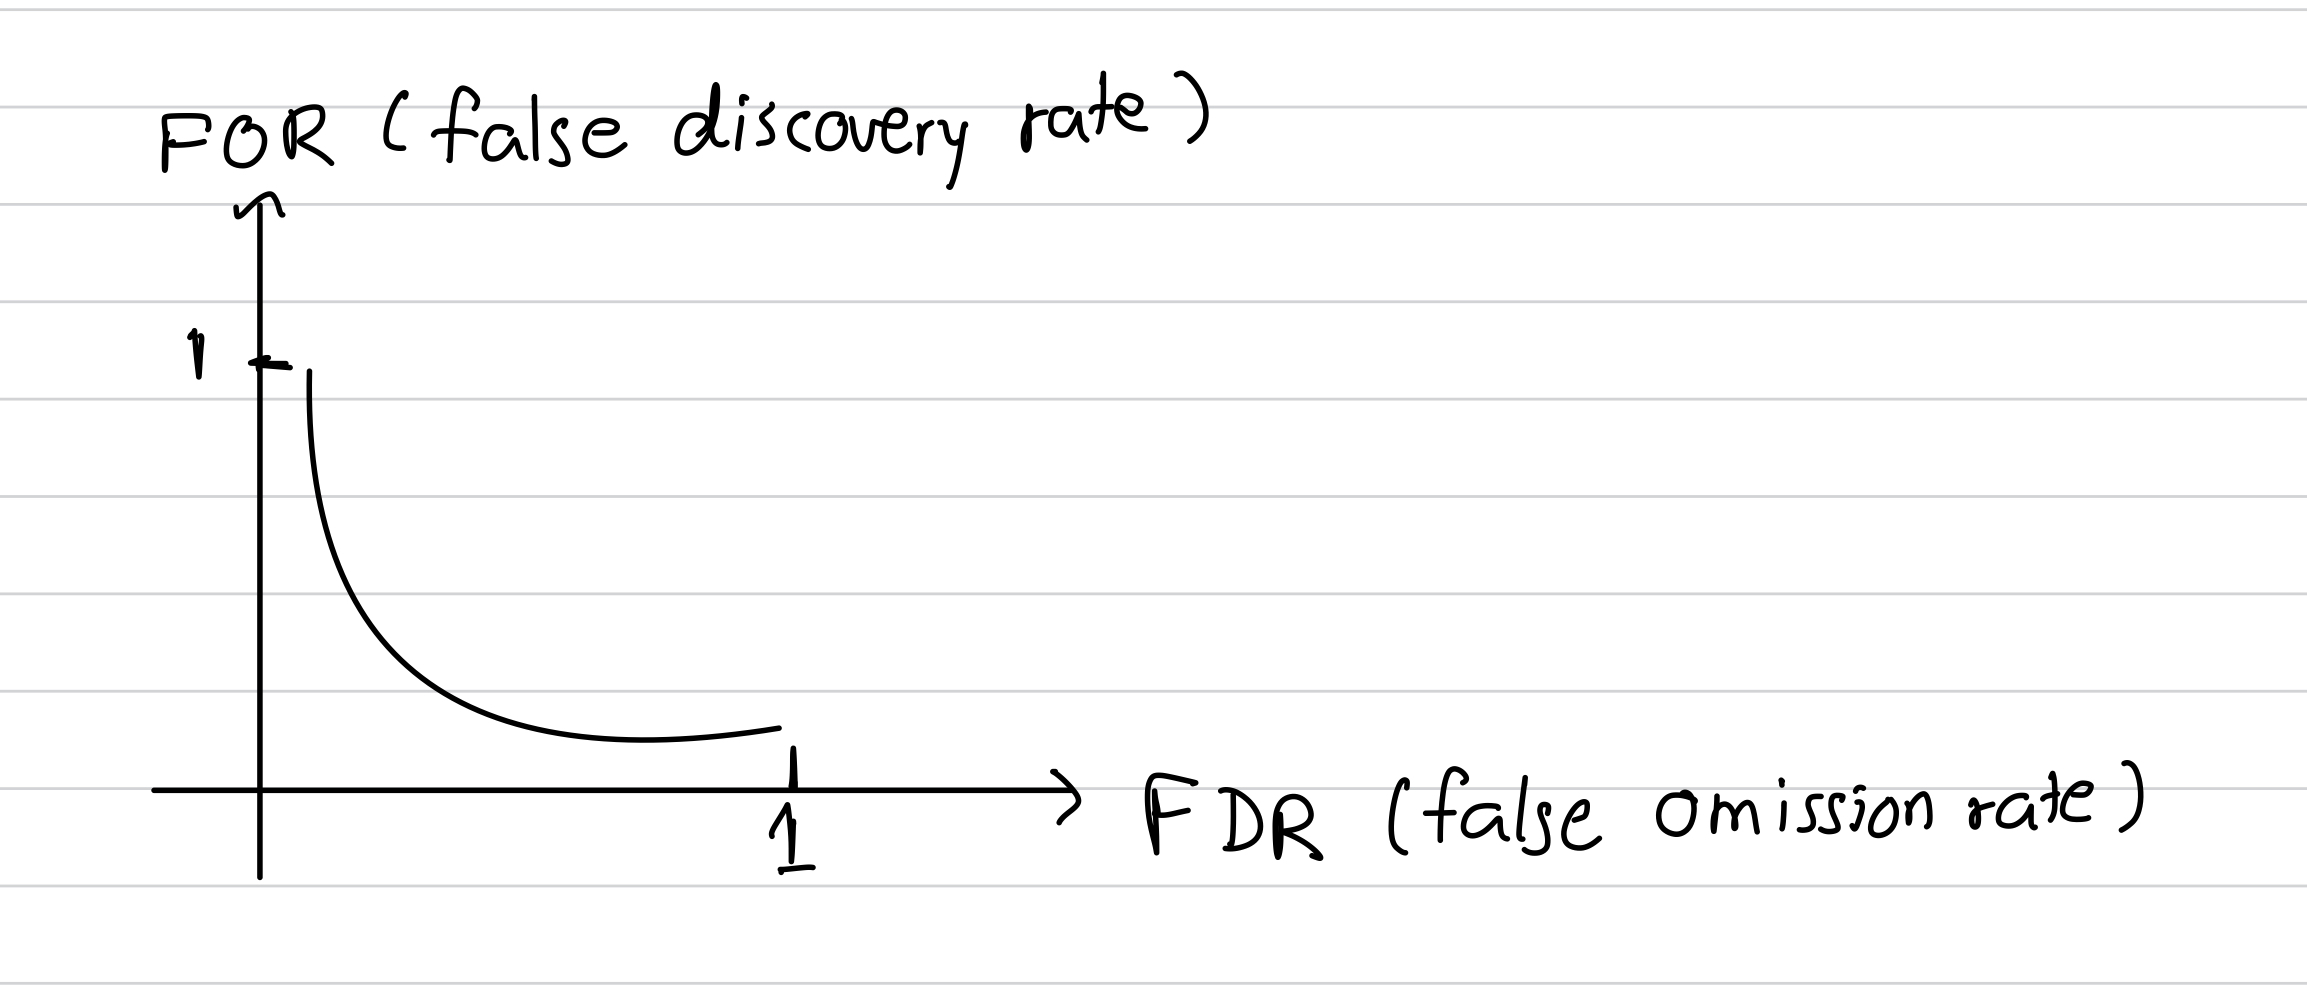
\includegraphics[width=0.75\linewidth]{imgs/img2.jpeg}
\end{figure}

FDR measures the proportion of mistakes where $\hat{y}$ = 1
FOR measures the proportion of mistakes where $\hat{y}$ = 0


\easysubproblem{Pick one point on your DET curve from the previous question. Explain a situation why you would employ this model.}\spc{3}

If I pick a point of 0.8 on the FDR, it means that 80\% of the prediction is false positive while about 10\% of prediction is false negative. I would employ this model in a situation where false negatives are very costly and I want to catch as many positives as possible.

\hardsubproblem{[MA] The line of random guessing on the ROC curve is the diagonal line with slope one extending from the origin. What is the corresponding line of random guessing in the DET curve? This is not easy...}\spc{5}
\end{enumerate}



\problem{These are some questions related to bias-variance decomposition. Assume the two assumptions from the notes about the random variable model that produces the $\delta$ values, the error due to ignorance.}

\begin{enumerate}
\easysubproblem{Write down (do not derive) the decomposition of MSE for a given $\x_*$ where $\mathbb{D}$ is assumed fixed but the response associated with $\x_*$ is assumed random.}\spc{1}
\[
\text{MSE}(\vec{x}_*) = \sigma^2 + \left( \text{Bias}[\vec{x}_*] \right)^2
\]


\easysubproblem{Write down (do not derive) the decomposition of MSE for a given $\x_*$ where the responses in $\mathbb{D}$ is random but the $\X$ matrix is assumed fixed and the response associated with $\x_*$ is assumed random like previously.}\spc{3}

\[
\text{MSE}[\vec{x}_*] = \sigma^2 + \left( \text{Bias}\left[ G(\vec{x}_*) \right] \right)^2 + \text{Var}\left[ G(\vec{x}_*) \right]
\]

\easysubproblem{Write down (do not derive) the decomposition of MSE for general predictions of a phenomenon where all quantities are considered random.}\spc{3}

\[
\text{MSE} = \sigma^2 + \mathbb{E}_{\vec{x}} \left[ \left( \text{Bias}\left[ G(\vec{x}_*) \right] \right)^2 \right] + \mathbb{E}_{\vec{x}} \left[ \text{Var}\left[ G(\vec{x}_*) \right] \right]
\]

\hardsubproblem{Why is it in (a) there is only a \qu{bias} but no \qu{variance} term? Why did the additional source of randomness in (b) spawn the variance term, a new source of error?}\spc{6}

In (a), the training data is fixed, so the model’s prediction at $\vec{x}_*$ is deterministic—there’s no variation across datasets, only bias and irreducible error contribute to MSE. In (b), the responses in the training data are random, making the learned model G itself random. This leads to variability in predictions at $\vec{x}_*$, introducing a new source of error: the variance of G($\vec{x}_*$).

\intermediatesubproblem{A high bias / low variance algorithm is underfit or overfit?}\spc{-0.5}

A high bias / low variance algorithm is underfit. High bias means the model is too simple to capture the underlying structure of the data, leading to systematic errors (misspecification). Low variance indicates that the model’s predictions do not change much across different training sets. For example, linear models often have high bias but low variance, making them prone to underfitting.

\intermediatesubproblem{A low bias / high variance algorithm is underfit or overfit?}\spc{-0.5}

A low bias / high variance algorithm is overfit. Low bias means the model can capture complex patterns in the data, but high variance indicates that its predictions are highly sensitive to the specific training data. This usually happens when the model is too complex, fitting noise rather than the true signal, which leads to overfitting.

\intermediatesubproblem{Explain why bagging reduces MSE for \qu{free} regardless of the algorithm employed.}\spc{6}

Bagging reduces MSE for free primarily by reducing variance without increasing bias. It works by training the model on multiple bootstrapped samples of the dataset, making each model g slightly different. Because these models are trained on different data, their errors are less correlated. When we average the predictions of these models, the variance of the ensemble decreases significantly, especially when the base models are unstable (high variance). This reduction in variance leads to a lower MSE without necessarily increasing bias, hence the improvement comes for free.

\intermediatesubproblem{Explain why RF reduces MSE atop bagging $M$ trees and specifically mention the target that it attacks in the MSE decomposition formula and why it's able to reduce that target.}\spc{5}

Random forests reduce MSE atop bagging by using a random subset of features at each split, which decorrelates the individual trees. This reduces the variance term in the MSE decomposition. It works because averaging predictions from less correlated models leads to a smaller overall variance since correlated errors don’t cancel out, but uncorrelated ones do. So, by lowering the correlation between trees, RF effectively lowers the model’s prediction variance across datasets, without increasing bias much.

\hardsubproblem{When can RF lose to bagging $M$ trees? Hint: think hyperparameter choice.}\spc{5}

Random forests can perform worse than bagging when the hyperparameter$ m_{\text{try}}$ is set too low—such as $m_{\text{try}} = 1$.
In this case, each split considers only one feature, which can severely limit the model’s ability to capture important interactions or  identify strong predictors. As a result, the trees become weak and the ensemble underfits the data, performing worse than standard bagging where all features are considered at each split.

\end{enumerate}



%\problem{These are some questions related to correlation-causation and interpretation of OLS coefficients.}
%
%\begin{enumerate}
%\easysubproblem{Consider a fitted OLS model for y with features $x_1$, $x_2$, \ldots, $x_p$. Provide the most correct interpretation of the quantity $b_1$ you can.}\spc{6}
%
%
%\easysubproblem{If $x$ and $y$ are correlated but their relationship isn't causal, draw a diagram below that includes $z$.}\spc{6}
%
%\easysubproblem{To show that $x$ is causal for $y$, what specifically has to be demonstrated? Answer with a couple of sentences.}\spc{4}
%
%\intermediatesubproblem{If we fit a model for y using $x_1$, $x_2$, \ldots, $x_7$, provide an example real-world illustration of the causal diagram for $y$ including the $z_1$, $z_2$, $z_3$.}\spc{5}
%
%
%\end{enumerate}
%
%
\problem{These are some questions related to missingness.}

\begin{enumerate}
\easysubproblem{[MA] What are the three missing data mechanisms? Provide an example when each occurs (i.e., a real world situation). We didn't really cover this in class so I'm making it a MA question only. This concept will NOT be on the exam.}\spc{3}

\easysubproblem{Why is listwise-deletion a \textit{terrible} idea to employ in your $\mathbb{D}$ when doing supervised learning?}\spc{3}

Listwise deletion is a terrible idea when the sample size n is small or the proportion of missing rows is large. It can lead to estimation errors because we lose valuable data, and to extrapolation errors if the missingness is not random — especially if rows with unique or informative patterns are dropped.


\easysubproblem{Why is it good practice to augment $\mathbb{D}$ to include missingness dummies? In other words, why would this increase oos predictive accuracy?}\spc{4}

It is good practice to augment $\mathbb{D}$ with missingness dummies because the pattern of missingness itself may carry predictive information. By including binary indicators for whether a value is missing, we allow the model to capture potential non-random missingness, which can improve out-of-sample (OOS) accuracy. It increases the feature set in a meaningful way and may reduce residual error if the pattern of missingness correlates with the target.

\easysubproblem{To impute missing values in $\mathbb{D}$, what is a good default strategy and why?}\spc{3}

A good default strategy is to use the MissForest algorithm to impute missing values. MissForest is a non-parametric method that uses random forests to predict missing entries based on all other observed features and, if available, the response variable. This works well because it can capture nonlinear relationships and interactions among variables. Since the features X and the response y are often correlated, MissForest can leverage these patterns to produce accurate imputations and improve out-of-sample predictive performance.


\end{enumerate}
%
%\problem{These are some questions related to lasso, ridge and the elastic net.}
%
%\begin{enumerate}
%\easysubproblem{Write down the objective function to be minimized for ridge. Use $\lambda$ as the hyperparameter.}\spc{2}
%
%\easysubproblem{Write down the objective function to be minimized for lasso. Use $\lambda$ as the hyperparameter.}\spc{3}
%
%\easysubproblem{We spoke in class about when ridge and lasso are employed. Based on this discussion, why should we restrict $\lambda > 0$?}\spc{3}
%
%\intermediatesubproblem{Why is lasso sometimes used a preprocessing step to remove variables that likely are not important in predicting the response?}\spc{3}
%
%
%\easysubproblem{Assume $\X$ is orthonormal. One can derive $\b_{\text{lasso}}$ in closed form. Copy the answer from the wikipedia page. Compare $\b_{\text{lasso}}$ to $\b_{\text{OLS}}$.}\spc{8}
%
%\intermediatesubproblem{Write down the objective function to be minimized for the elastic net. Use $\alpha$ and $\lambda$ as the hyperparameters.}\spc{3}
%
%\easysubproblem{We spoke in class about the concept of the elastic net. Based on this discussion, why should we restrict $\alpha \in (0, 1)$?}\spc{3}
%
%\end{enumerate}

\problem{These are some questions related to gradient boosting. The final gradient boosted model after $M$ iterations is denoted $G_M$ which can be written in a number of equivalent ways (see below). The $g_t$'s denote constituent models and the $G_t$'s denote partial sums of the constituent models up to iteration number $t$. The constituent models are \qu{steps in functional steps} which have a step size $\eta$ and a direction component denoted $\tilde{g}_t$. The directional component is the base learner $\mathcal{A}$ fit to the negative gradient of the objective function $L$ which measures how close the current predictions are to the real values of the responses:

\beqn
G_M &=& G_{M-1} + g_M \\
&=& g_0 + g_1 + \ldots + g_M \\
&=& g_0 + \eta \tilde{g}_1 + \ldots + \eta \tilde{g}_M \\
&=& g_0 + \eta \mathcal{A}\parens{\left<\X, -\nabla L(\y, \yhat_1)\right>, \mathcal{H}} + \ldots + \eta \mathcal{A}\parens{\left<\X, -\nabla L(\y, \yhat_M)\right>, \mathcal{H}} \\
&=& g_0 + \eta \mathcal{A}\parens{\left<\X, -\nabla L(\y, g_1(\X))\right>, \mathcal{H}} + \ldots + \eta \mathcal{A}\parens{\left<\X, -\nabla L(\y, g_M(\X))\right>, \mathcal{H}} 
\eeqn}

\begin{enumerate}
\easysubproblem{From a perspective of only multivariable calculus, explain gradient descent and why it's a good idea to find the minimum inputs for an objective function $L$ (in English).}\spc{2.5}

Gradient descent is an algorithm where we start with an initial point on a graph (in 1D or on a surface in higher dimensions) and move step by step toward the minimum of a function. At each step, we use the gradient (slope) of the loss function and adjust by a small amount called the learning rate. Over time, this process leads us closer to the point that minimizes the loss.

It’s a good idea to find the minimum inputs for an objective function L because minimizing L reduces the model’s residuals (errors). In other words, each step helps improve our predictions by lowering the difference between predicted and true values.

\easysubproblem{Write the mathematical steps of gradient boosting for supervised learning below. Use $L$ for the objective function to keep the procedure general. Use notation found in the problem header. 
}\spc{8}

\begin{enumerate}
    \item Begin at \( G_0 = g_0 \), the default.
    
    \item Compute the direction that improves loss:
    \[
    \mathcal{A}(\langle X, -\nabla L(\vec{y}, \vec{\hat{y}}_0) \rangle, \mathcal{H})
    \]
    That is, run the algorithm on data \( X \), but fit on the loss of \( \vec{\hat{y}} \).
    
    \item Move by amount:
    \[
    g_1 = \eta \cdot \mathcal{A}(\langle X, -\nabla L(\vec{y}, \vec{\hat{y}}_0) \rangle, \mathcal{H})
    \]
    where \( \eta \) is the learning rate.
    
    \item Compute a better approximation:
    \[
    G_1 = g_0 + g_1
    \]
    
    \item Compute a second approximation:
    \[
    G_2 = g_0 + g_1 + \eta \cdot \mathcal{A}(\langle X, -\nabla L(\vec{y}, \vec{\hat{y}}_1) \rangle, \mathcal{H})
    \]
    
    \item Compute the \( m \)-th approximation:
    \[
    G_m = g_0 + g_1 + \cdots + g_{m-1} + \eta \cdot \mathcal{A}(\langle X, -\nabla L(\vec{y}, \vec{\hat{y}}_{m-1}) \rangle, \mathcal{H})
    \]
    
    \item Final model:
    \[
    g_{\text{boost}} = G_m
    \]
\end{enumerate}

\easysubproblem{For regression, what is $g_0(\x)$?}\spc{1}

$\bar{y}$

\easysubproblem{For probability estimation for binary response, what is $g_0(\x)$?}\spc{1}

$\bar{y}$, the proportion of 1's in $\mathbb{D}$ of the n observation

\intermediatesubproblem{What are all the hyperparameters of gradient boosting? There are more than just two.}\spc{3}

Learning Rate $\eta$, number of iteration $M$, since we are using shallow tree, $N_0$ large, depending on the response $y$ we use different loss function.


\easysubproblem{For regression, rederive the negative gradient of the objective function $L$.}\spc{2}

For \( y \in \mathbb{R} \) and 
\[
L(\vec{y}, \vec{\hat{y}}) = \text{SSE} = \sum_{i=1}^n (y_i - \hat{y}_i)^2,
\]

\[
-\nabla L(\vec{y}, \vec{\hat{y}}) 
= - 
\begin{bmatrix}
\frac{\partial L}{\partial \hat{y}_1} \\
\vdots \\
\frac{\partial L}{\partial \hat{y}_n}
\end{bmatrix}
= -
\begin{bmatrix}
-(y_1 - \hat{y}_1) \\
\vdots \\
-(y_n - \hat{y}_n)
\end{bmatrix}
= 2(\vec{y} - \vec{\hat{y}}) = 2\vec{e}
\]

\[
g_1 = \eta \cdot \mathcal{A}(\langle X, 2\vec{e} \rangle, \mathcal{H})
\]



\easysubproblem{For probability estimation for binary response, rederive the negative gradient of the objective function $L$.}\spc{12}

The target is \( P(Y = 1 \mid \vec{x}) \).

Logistic Link Function
\[
\phi(u) = \frac{e^u}{1 + e^u}
\]

Log Odds
Let \( \hat{y}_i = \ln\left( \frac{\hat{p}_i}{1 - \hat{p}_i} \right) \Rightarrow \hat{p}_i = \frac{e^{\hat{y}_i}}{1 + e^{\hat{y}_i}} \)

\[
1 - \hat{p}_i = 1 - \frac{e^{\hat{y}_i}}{1 + e^{\hat{y}_i}} = \frac{1}{1 + e^{\hat{y}_i}}
\]

Probability of Data
\[
P(\vec{y}, \hat{\vec{p}}) = \prod_{i=1}^n \hat{p}_i^{y_i} (1 - \hat{p}_i)^{1 - y_i}
\]

Substitute \( \hat{p}_i = \frac{e^{\hat{y}_i}}{1 + e^{\hat{y}_i}} \), then:
\[
P(\vec{y}, \hat{\vec{p}}) = \prod_{i=1}^n \left( \frac{e^{\hat{y}_i}}{1 + e^{\hat{y}_i}} \right)^{y_i} \left( \frac{1}{1 + e^{\hat{y}_i}} \right)^{1 - y_i}
= \prod_{i=1}^n \frac{e^{y_i \hat{y}_i}}{1 + e^{\hat{y}_i}} = P(\vec{y}, \hat{\vec{y}})
\]

Log-Likelihood
Maximizing probability is equivalent to maximizing the log-probability.

\[
L(\vec{y}, \hat{\vec{y}}) = \ln \left( P(\vec{y}, \hat{\vec{y}}) \right)
= \sum_{i=1}^n \ln\left( \frac{e^{y_i \hat{y}_i}}{1 + e^{\hat{y}_i}} \right)
= \sum_{i=1}^n \left( y_i \hat{y}_i - \ln(1 + e^{\hat{y}_i}) \right)
\]

Gradient of the Loss
\[
-\nabla L(\vec{y}, \hat{\vec{y}}) = -
\begin{bmatrix}
\frac{\partial L}{\partial \hat{y}_1} \\
\vdots \\
\frac{\partial L}{\partial \hat{y}_n}
\end{bmatrix}
= -
\begin{bmatrix}
y_1 - \frac{e^{\hat{y}_1}}{1 + e^{\hat{y}_1}} \\
\vdots \\
y_n - \frac{e^{\hat{y}_n}}{1 + e^{\hat{y}_n}}
\end{bmatrix}
= \vec{y} - \vec{p} = \vec{e}
\]

So the residuals \( \vec{e} \) are:
\[
\vec{e} = \vec{y} - \vec{p}
\]

\hardsubproblem{For probability estimation for binary response scenarios, what is the unit of the output $G_M(\x_\star)$?}\spc{2}

The unit of the output is probability of being 1.

\easysubproblem{For the base learner algorithm $\mathcal{A}$, why is it a good idea to use shallow CART (which is the recommended default)?}\spc{3}

It is because "weak learner" eg. shadow tree. has high bias and low variance but flexible enough so that a sum of many can be complex. Also, Cov[$g_i, g_j$]'s are small since they are weak in different ways. Thus, Var[$g_{Boost}$] is small. Begin with lo variance and as M increases Bias will decrease.

\hardsubproblem{For the base learner algorithm $\mathcal{A}$, why is it a bad idea to use deep CART?}\spc{2}

Using deep CART as the base learner $\mathcal{A}$ is a bad idea because deep trees have high variance and tend to overfit the training data. Boosting works best with weak learners that have high bias and low variance; using strong learners like deep CART defeats this purpose and increases the risk of overfitting. Moreover, since boosting sums models rather than averaging them, it cannot effectively reduce variance when the base learners are deep trees.

\hardsubproblem{For the base learner algorithm $\mathcal{A}$, why is it a bad idea to use OLS for regression (or logistic regression for probability estimation for binary response)?}\spc{2}

Using OLS for regression or logistic regression for binary classification as the base learner $\mathcal{A}$ is a bad idea because they are strong learners with low bias. Boosting is designed to iteratively improve weak learners with high bias and low variance. If you use strong learners, boosting has little room to improve, and it can lead to overfitting or redundancy. Boosting works best when each base learner only captures a small part of the signal.

\hardsubproblem{If $M$ is very, very large, what is the risk in using gradient boosting even using shallow CART as the base learner (the recommended default)?}\spc{2}

If M (the number of boosting iterations) is very large, even with shallow CART as the base learner, the model can overfit. Boosting keeps adding trees to reduce training error, and with enough iterations, it can start fitting noise in the data. This leads to poor generalization on new, unseen data. 

\hardsubproblem{If $\eta$ is very, very large but $M$ reasonably correctly chosen, what is the risk in using gradient boosting even using shallow CART as the base learner (the recommended default)?}\spc{2}

If $\eta $(the learning rate) is very large, even with a reasonable number of iterations M and shallow CART as the base learner, the updates can overshoot the minimum. This causes the model to jump around rather than converge smoothly, leading to instability and poor performance. It may fail to minimize the loss properly, resulting in underfitting or erratic predictions.

\end{enumerate}




\end{document}






